\begin{table}[!htb]
    \label{table:generalComparing}
    \rowcolors{2}{white}{gray!20}
    \tablesettings{Vergleich der Auswahlmöglichkeiten}
    \footnotesize
    % \scalebox{0.8}{
    \begin{threeparttable}
        \begin{tabular}{ l || c | c | c | c }
            Kriterium & Buttons & Select & List & Country Input \\
            \hline % column for new goal input
            \hline
            \tbbr{Optimale \\ Anzahl Elemente} & 1 – 3 & 7 ± 2 & 70 ± 20 & ca. 250 \\
            \hline
            Alternativ-Name & Links & Choice Input & Combo Box & keine \\
            \hline
            Falsche Auswahl & \xmark & \xmark & \cmark & \xmark \\
            \hline
            Multi-Auswahl & \cmark & \cmark & \xmark & \xmark \\
            \hline
            Readonly & \cmark & \xmark & \cmark & \xmark \\
            \hline
            Disabled & \cmark & \cmark & \cmark & \xmark \\
            \hline
            Werte-Typ & Skalar & Skalar & Skalar & Objekt \\
            \hline
            \tbbr{Interaktions-\\möglichkeit} & sehr begrenzt & gut & gut & gut \& konsistent \\
            \hline
            \tbbr{Aktion bei \\ Symbol-Eingabe} & keine & Suche\tnote{2} & Filter\tnote{1} & Suche\tnote{2} \\
            \hline
            Merkmal & direkter Überblick & fixe Optionen & Eingabehilfe & \tbbr{Speziell für \\ Länderauswahl} \\
            \hline
            Anwendung & \tbbr{Navigationslink, \\ Formularbuttons} & \tbbr{Formularfeld \\ mit begrenzter \\ Auswahl} & \tbbr{Filterbare Liste, \\ Suchergebnis} & \tbbr{Länderauswahl \\ im Formular} \\
            % \hline % own table for browsers
            % Bilder 
            %     & 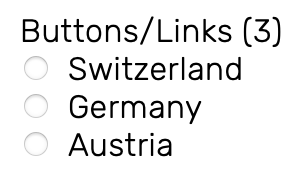
\includegraphics[width=28mm,scale=0.5]{radios-example.png} 
            %         \captionof{figure}{Radio Buttons mit 3 Werten}
            %     & 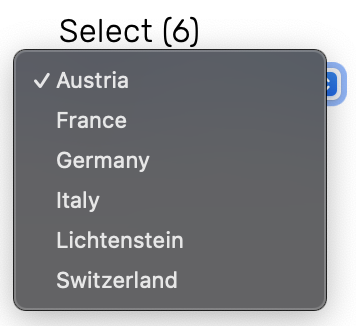
\includegraphics[width=33mm,scale=0.5]{select-open-example.png} 
            %         \captionof{figure}{Select mit 6 Werten}
            %     & 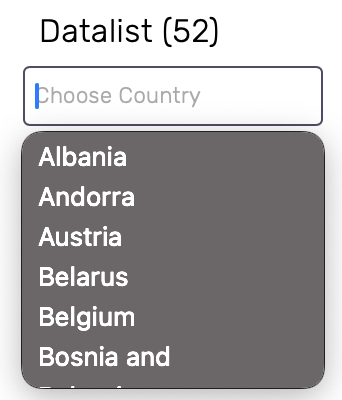
\includegraphics[width=33mm,scale=0.5]{datalist-example.png} 
            %         \captionof{figure}{Datalist mit 52 Werten}
            %     & 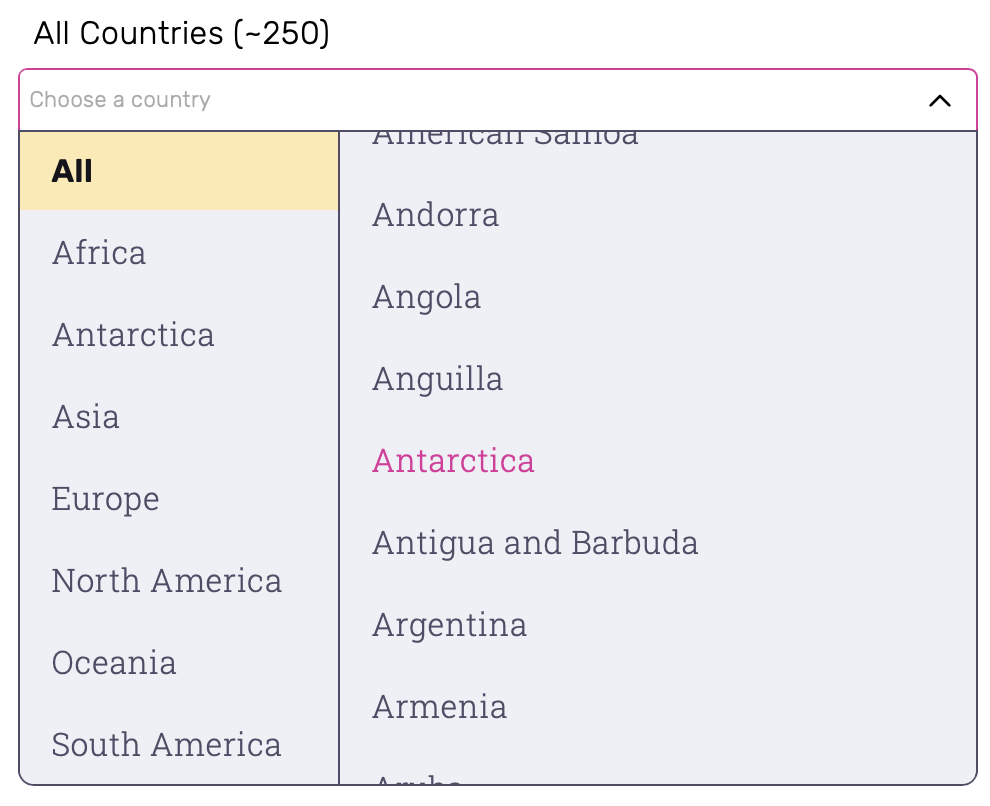
\includegraphics[width=33mm,scale=0.5]{country-list-example.png} 
            %         \captionof{figure}{Country Input}
            % \\
        \end{tabular}
        \begin{tablenotes}
            \scriptsize
            \item[1] Filter: Liste verändern je nach Anzahl passender Werte
            \item[2] Suche: Liste unverändert; Erster zu der Eingabe passender Wert aus der Liste     
        \end{tablenotes}
    \end{threeparttable}
    % }
\end{table}
